\documentclass{article}
\usepackage[utf8]{inputenc}
\usepackage{lipsum} % Package used to generate dummy text
\usepackage{tocloft} % Package used to format table of contents
\usepackage{titlesec} % Package used to format titles
\usepackage{geometry} 
\usepackage{graphicx}%
\usepackage{titlesec}Package used to adjust page layout

% Formatting titles
\titleformat{\section}u
  {\normalfont\Large\bfseries}{\thesection}{1em}{}
\titleformat{\subsection}
  {\normalfont\large\bfseries}{\thesubsection}{1em}{}
\titleformat{\subsubsection}
  {\normalfont\normalsize\bfseries}{\thesubsubsection}{1em}{}

% Formatting table of contents
\renewcommand{\cftsecfont}{\normalfont}
\renewcommand{\cftsecpagefont}{\normalfont}
\renewcommand{\cftsubsecfont}{\normalfont}
\renewcommand{\cftsubsecpagefont}{\normalfont}
\renewcommand{\cftsubsubsecfont}{\normalfont}
\renewcommand{\cftsubsubsecpagefont}{\normalfont}
\date{} 

\begin{document}
\renewcommand{\contentsname}{Table des matières}
\tableofcontents

\clearpage


\maketitle

\section * {Introduction}
\addcontentsline{toc}{section}{Introduction}
% Introduction du rapport de projet, contexte, objectifs, etc.
Lorsque nous entreprenons un voyage, ou bien voulons-nous nous déplacer d’un lieu à un autre, nous sommes guidés par l’envie de nous déplacer de manière la plus sûre possible, en un laps de temps suffisamment court, sans oublier la curiosité, l’envie de découvrir de nouveaux horizons, et le désir de vivre des expériences inoubliables. Mais comment planifier efficacement notre itinéraire pour maximiser notre temps et profiter au maximum de chaque étape ? 

Dans cette optique, le projet « My way » vise à explorer l’art de créer des itinéraires, et le suivi des voyages bien structurés. Nous allons plonger dans l’élaboration d’itinéraires détaillés, étape par étape, en tenant compte des intérêts, des contraintes et des préférences de chaque voyageur. Que vous soyez un utilisateur lambda, un voyageur, un blogueur ou un professionnel du tourisme, la capacité à concevoir des itinéraires et le suivi en temps réel du déplacement pertinents est essentielle.


Nous entamons cette démarche en procédant à une analyse statistique détaillée afin de mieux appréhender les défis et les enjeux associés à la mobilité urbaine. Ensuite, nous explorerons les différentes fonctionnalités potentielles nécessaires pour résoudre ce problème, en tenant compte des besoins des utilisateurs et des contraintes technologiques. Nous aborderons également l’importance du sous-secteur dans la transformation digitale du pays, mettant en lumière les avantages économiques, sociaux et environnementaux que pourrait apporter une solution innovante. Par la suite, nous examinerons les scénarios d’utilisation possibles, les acteurs impliqués et les implications sur l’environnement technique nécessaire au déploiement de l’application. Enfin, nous proposerons une modélisation mathématique du problème à l’aide de la théorie des graphes, offrant ainsi une approche structurée et rigoureuse pour résoudre efficacement les défis de gestion et de parcours d’itinéraires.

\newpage

\section{Contexte}
% Présentation du contexte du projet

La ville de Yaoundé, capitale du Cameroun, connaît une croissance démographique rapide avec environ 4,3 millions d’habitants. Comme de nombreuses grandes villes d’Afrique subsaharienne, Yaoundé est confrontée à des défis liés à la mobilité urbaine. Actuellement, les modes de déplacement prédominants sont les taxis collectifs (40 \% des déplacements) et la marche à pied (33 \% des déplacements).

Cependant, le réseau viaire de Yaoundé présente des limites en raison d’un manque d’entretien, d’une gestion sous-optimale des intersections et d’une occupation non contrôlée de la voirie. Face à ces enjeux, le projet “My Way” vise à améliorer la mobilité urbaine et à faciliter les déplacements quotidiens des habitants.

\section{Méthodologie}
% Description de la méthodologie utilisée dans le projet
 Analyse de la mobilité urbaine à Yaoundé :
Nous avons commencé par une analyse approfondie de la situation actuelle de la mobilité urbaine à Yaoundé, en nous concentrant sur les aspects architecturaux de la voirie urbaine, l'évolution des modes de transports dans la ville, y compris la montée des taxis collectifs et des motos-taxis, ainsi que les problèmes actuels de mobilité dans la ville, tels que la congestion routière et les défis liés à la gestion des infrastructures.

Étude des fonctionnalités nécessaires pour une application de transport urbain :
Nous avons ensuite examiné les fonctionnalités essentielles qu'une application de transport urbain devrait posséder pour répondre efficacement aux besoins des habitants de Yaoundé, en tenant compte des contraintes technologiques et des préférences des utilisateurs.

Impact de la transformation digitale au Cameroun :
Nous avons évalué l'impact de la transformation digitale sur le paysage urbain de Yaoundé, en mettant en lumière les tendances telles que l'explosion du commerce électronique, l'utilisation croissante des données et les changements dans le paysage concurrentiel, ainsi que les implications environnementales, sociales et économiques associées.

Illustration de la criticité du problème de mobilité :
Nous avons illustré l'importance critique du problème de mobilité dans la ville de Yaoundé en examinant les données démographiques, les statistiques de déplacement et les exemples concrets de situations de mobilité problématiques dans la ville.

Identification des acteurs et de l'environnement technique :
Nous avons identifié les acteurs clés impliqués dans la gestion de la mobilité urbaine à Yaoundé, ainsi que l'environnement technologique nécessaire au développement et au déploiement d'une solution innovante pour améliorer la mobilité.

Analyse des ressources et des contraintes :
Nous avons analysé les ressources disponibles et les contraintes potentielles à prendre en compte lors de la mise en œuvre de solutions pour améliorer la mobilité urbaine à Yaoundé.

Exploration des aspects de régulation, des contraintes opérationnelles et des solutions digitales :
Nous avons examiné les aspects réglementaires et opérationnels liés à la gestion de la mobilité urbaine, ainsi que les solutions digitales pouvant contribuer à la résolution des défis rencontrés.

Modélisation mathématique du problème :
Nous avons proposé une modélisation mathématique du problème de mobilité urbaine à l'aide de la théorie des graphes, offrant ainsi une approche structurée pour résoudre efficacement les défis de gestion des itinéraires et des déplacements.

Après avoir suivi les étapes précédentes, nous avons développé une application web pour résoudre le problème d'itinéraire et de suivi d'un voyage. Cette application vise à offrir plusieurs fonctionnalités afin de répondre aux besoins variés des utilisateurs en matière de déplacement. Les principales fonctionnalités de cette application sont les suivantes :

\begin{itemize}
    \item \textbf{Suivi en temps réel des déplacements :} Les utilisateurs peuvent suivre en temps réel leurs déplacements grâce à la géolocalisation, ce qui leur permet de planifier leurs trajets de manière efficace et d'adapter leurs itinéraires en cas de besoin.
    
    \item \textbf{Proposition d'itinéraires quotidiens :} L'application propose des itinéraires quotidiens aux utilisateurs en fonction de leurs préférences et de leurs besoins. Les utilisateurs peuvent filtrer les itinéraires en fonction de critères tels que la distance, le temps de déplacement, les tarifs des différents moyens de transport disponibles, etc.
    
    \item \textbf{Itinéraires personnalisés :} Pour les utilisateurs souhaitant se déplacer d'un point A à un point B en passant par des points intermédiaires (C, D, etc.), l'application propose des itinéraires personnalisés qui prennent en compte ces points de passage.
\end{itemize}

Grâce à ces fonctionnalités, notre application web vise à simplifier et à améliorer l'expérience de déplacement des utilisateurs à Yaoundé, en leur offrant des solutions adaptées à leurs besoins spécifiques.



 \section{Analyse de la mobilité urbaine et interurbaine et cas particulier dans la ville de Yaoundé}

La mobilité urbaine et interurbaine a été et demeure toujours un sujet d'intérêt, un problème qui a toujours suscité l'attention, vu son importance dans le développement économique d'un État. Elle dépend fortement d'un ensemble de facteurs, lesquels facteurs retiendront notre attention dans l'analyse du cas de la ville de Yaoundé qui suit.

\subsection{Architecture routière de ville de Yaoundé}

\begin{figure}[h]
    \centering
    \includegraphics[width=0.5\linewidth]{Images/Reseau_Routier_Yaoundé.png}
    \caption{Réseau routier - Yaoundé}
    \label{fig:reseau_routier}
    \cite{mfoulou2016mobilite}
\end{figure}

Au vu de la carte \ref{fig:reseau_routier} ci-dessus, on constate que le réseau routier de la ville de Yaoundé a plus ou moins une structure en étoile, centrée au niveau du centre ville et principalement du lieu dit: poste centrale. 
C'est à juste titre (comme le montre l'illustration \ref{fig:trafic_routier} en dessous, qu'on observe un trafic intense au niveau des zones proches du centre ville.

\begin{figure}[h]
    \centering
    \includegraphics[width=0.72\linewidth]{Images/Traffic_Routier_Yaoundé.png}
    \caption{Trafic routier - Yaoundé}
    \label{fig:trafic_routier}
    \cite{mfoulou2016mobilite}
\end{figure}

On déplore alors cette architecture, qui favorise des embouteillages chroniques et très souvent des accidents.
Toutefois, un réseau routier basé sur plusieurs pôles au lieu d'un seul, aurait amélioré la situation.

\subsection{Évolution des modes de transports dans la ville de Yaoundé}

Les moyens de transports dans la ville de Yaoundé, ont fortement évolués depuis la crise économique dont a été victime le Cameroun dans les années 80. 

\subsection{La SOTUC et son déclin}

La SOTUC\footnote{Société des transports urbains du Cameroun.
} a été créée en 1973 pour assurer le transport public urbain à Yaoundé. \emph{A l'époque}, elle était le principal opérateur de transport avec une flotte de bus importante. Cependant, la SOTUC a connu un déclin progressif au fil des années. \emph{En 2023}, la société ne disposait que d'une centaine de bus en état de marche, ce qui est largement insuffisant pour répondre aux besoins de la population croissante de Yaoundé.

\subsection{L'émergence des motos-taxis}

Face à l'insuffisance de la SOTUC, les motos-taxis, communément appelées "clandos", ont fait leur apparition dans les années 1990. \emph{Elles sont rapidement devenues le mode de transport dominant à Yaoundé}, en raison de leur flexibilité et de leur coût abordable. On estime aujourd'hui qu'il y a plus de 200 000 motos-taxis en activité à Yaoundé.

Dès lors les déplacements dans la ville de Yaoundé se font exclusivement via les taxis en plein coeur de la ville, et via les motos pour les coins reculés et les quartiers périphériques.

\subsection{État actuel de la mobilité dans la ville de Yaoundé}
\begin{figure}[h]
    \centering
    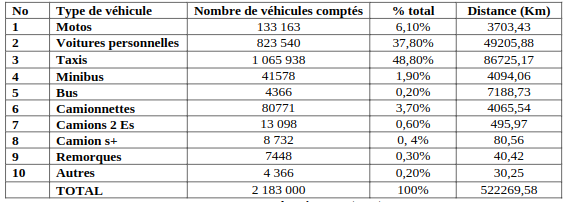
\includegraphics[width=0.8\linewidth]{Images/Repartition_Trafic_Par_Vehicule.png}
    \caption{Répartition du trafic routier à Yaoundé}
    \label{fig:repartition_trafic}
    \cite{mfoulou2016mobilite}
\end{figure}

Les statistiques sont claires. Les citoyens de la ville de Yaoundé se déplace exclusivement en taxi
 ou en moto. Les facteurs déterminants pour le choix de mobilité à Yaoundé incluent l’accessibilité, la densité de la zone d’origine, et le motif de déplacement. L’accessibilité influence négativement l’usage de la moto et du taxi, mais positivement celui du bus, minibus et voiture personnelle. Les zones denses encouragent l’usage de la moto en raison de l’absence d’aménagements publics et de la demande élevée en mobilité, tandis que la densité a un impact négatif sur le choix du taxi dû à la congestion. Le motif de déplacement influence positivement tous les modes de transport, avec une préférence moindre pour la moto pour se rendre au travail. La localisation du logement par rapport aux grands axes radiaux et la distance du goudron sont également cruciales, tandis que l’heure de déplacement n’affecte pas l’usage de la moto ou de la voiture personnelle.

 Mais quelles peuvent être les conséquences de ces choix de mobilité ?

 \subsection{Problèmes de mobilité dans la ville de Yaoundé}

Vu la structure centrée de la ville de Yaoundé et de l'usage exclusif de moyens de transports à faible capacité (taxis et motos), celle-ci est très fréquemment le théâtre de congestion et de difficultés de déplacements, ce qui est un problème qui prend de plus en plus de l'ampleur. D'autant plus que l'usage des bus (plus appropriés pour résoudre le problème), ne se ressent quasiment plus.

Face à une ville avec une structure inadéquate pour les transports de masse, et très souvent aussi à l'incivisme des conducteurs d'automobile, une plate-forme accessible à tous, qui permettrait de repartir de manière uniforme le trafic dans la ville s'avère alors utile.,Mais alors, quelles fonctionnalités devrait avoir une telle solution en vue de résoudre optimalement le problème posé, et en vue de mieux s'intégrer dans la vie de tous les jours ? C'est ce dont nous en parlerons dans la suite 

\section{Fonctionnalités d'une application pouvant transformer le secteur du transport urbain et inter-urbain}

\begin{enumerate}
\item \textbf{Calcul d'itinéraire intelligent :}
L’application devrait permettre aux utilisateurs de saisir leur point de départ et leur destination, puis générer une liste d'itinéraires classés par ordre d'optimalité en tenant compte des modes de transport disponibles (bus, taxis, moto-taxis, etc.). L'application pourrait aussi proposer le calcul d'itinéraire par filtre (distance, coût, surcharge de la route, état de la route, etc.).
\item \textbf{Calcul d'itinéraire en temps réel :}
Le calcul d'itinéraire optimal pour l'utilisateur devrait pouvoir se faire automatiquement en temps réel lorsqu'il se déplace par rapport à son point d'arrivée.

\item \textbf{Cartographie détaillée :}
- Afficher des cartes interactives avec des points d’intérêt, des arrêts de transport, des stations-service, etc.
- Proposer des vues 3D pour faciliter la navigation.

\item \textbf{Informations en temps réel :}
Fournir des mises à jour en temps réel sur les conditions de circulation, les retards et les incidents sur les routes pour permettre aux utilisateurs de planifier leurs déplacements en conséquence, et même de changer d'itinéraire en cas de problème.

\item \textbf{Indications précises :}
Fournir des indications précises et détaillées, y compris les points d'intérêt, les intersections, les changements de direction, etc., pour aider les utilisateurs à naviguer facilement dans la ville.

\item \textbf{Navigation hors ligne :}
Permettre aux utilisateurs de télécharger des cartes et des itinéraires pour une navigation hors ligne dans les zones où la connectivité Internet est limitée.

\item \textbf{Collaboration avec d'autres services :}
L'application devrait permettre de collaborer avec d'autres services tels que la collecte des clients sur un itinéraire, le suivi d'un voyage, et autres.

\item \textbf{Statistiques de déplacement et IA :}
L'application pourrait enregistrer les différentes données statistiques de déplacement de ses utilisateurs qui pourraient aider à des prises de décision et même aux prédictions sur le temps de parcours, la surcharge de certaines routes, et proposer un modèle d'intelligence artificielle pour différentes prévisions et conseils.

\item \textbf{Suivi personnalisé et Synchronisation avec le calendrier :}
L'application devrait pouvoir utiliser les données et préférences de déplacement d'un utilisateur pour lui proposer un service client personnalisé automatique et lui offrir des conseils ; cette partie peut également être basée sur l'IA. L’application devrait également utiliser le calendrier des utilisateurs pour gérer les itinéraires de voyage en fonction de leur emploi du temps.

\item \textbf{Proposition de réservations :}
Afin d'éviter les désagréments souvent causés par des routes bloquées par le gouvernement lors des journées nationales ou lors du déplacement du chef de l'État, l'application devrait pouvoir permettre au gouvernement de réserver des routes à cet effet afin d'éviter de pénaliser les usagers et d'exploiter au mieux les routes libres dans ces situations.

\item \textbf{Partage d’itinéraire :}
Permettre aux utilisateurs de partager facilement leur itinéraire de voyage avec des amis ou des membres de la famille.

\item \textbf{Intégration des avis :}
L'application devrait incorporer des avis et des recommandations d'autres voyageurs sur des étapes spécifiques de l'itinéraire.
\end{enumerate}

\section{Impact de la Transformation Digitale au Cameroun}

Entre 2020 et 2021, le Cameroun a enregistré une croissance impressionnante de 12\% du nombre d'abonnements internet, portant le total à 12,5 millions d'abonnés. Cette expansion témoigne de l'engouement croissant de la population pour les services en ligne, reflétant ainsi une évolution significative des comportements et des attentes des consommateurs.

Un chiffre frappant est celui indiquant que 70\% des Camerounais utilisent désormais internet pour leurs communications personnelles, démontrant ainsi l'intégration profonde des outils numériques dans la vie quotidienne des citoyens. Cette utilisation généralisée d'internet comme canal de communication renforce l'idée d'une société de plus en plus interconnectée, où les échanges d'informations et les interactions sociales se déroulent de manière numérique.

Parallèlement, le marché des services digitaux au Cameroun a connu une croissance exponentielle, avec une évaluation atteignant 200 milliards de FCFA en 2023. Cette progression témoigne de l'essor d'un écosystème digital dynamique, où les opportunités commerciales et entrepreneuriales sont en constante expansion.

Dans ce contexte évolutif, l'importance d'une application de transport dans la ville de Yaoundé ne peut être surestimée. En exploitant les possibilités offertes par la digitalisation, une telle application peut contribuer de manière significative à la modernisation des infrastructures urbaines et à l'amélioration de la qualité de vie des habitants. Elle offre également une occasion unique de répondre aux besoins de mobilité croissants de la population tout en favorisant une gestion plus efficace et durable des ressources de la ville.
\subsection{Explosion du E-commerce}

La digitalisation du transport est étroitement liée à l'essor du commerce électronique. Avec la croissance exponentielle des achats en ligne, la demande de services de livraison efficaces et rapides est en constante augmentation. Les solutions numériques permettent d'optimiser les processus de livraison, de réduire les coûts logistiques et d'améliorer la satisfaction client en offrant un suivi en temps réel des colis.

\subsection{Utilisation Croissante de la Data}

Le secteur du transport génère une quantité massive de données, allant des itinéraires aux temps de transit en passant par les préférences des clients. La digitalisation permet une analyse approfondie de ces données, offrant des informations précieuses pour optimiser les itinéraires, planifier les opérations de transport et améliorer la gestion des stocks. Ces données alimentent également les algorithmes d'intelligence artificielle et de machine learning, permettant des prévisions plus précises et une prise de décision plus éclairée.

\subsection{Évolution du Paysage Concurrentiel}

L'ouverture à la concurrence et l'émergence de start-ups innovantes dans le secteur du transport incitent les entreprises établies à repenser leurs modèles commerciaux. La digitalisation offre des opportunités pour se différencier en offrant des services plus personnalisés, en améliorant l'expérience client et en adoptant des pratiques plus durables. Les entreprises qui investissent dans des technologies de pointe voient souvent une amélioration significative de leur compétitivité sur le marché.

\subsection{Impact Environnemental et Sociétal}

Le secteur du transport est l'un des principaux contributeurs aux émissions de gaz à effet de serre. La digitalisation offre des moyens de réduire cet impact en optimisant les itinéraires, en favorisant le covoiturage et en encourageant l'adoption de véhicules électriques et de carburants alternatifs. De plus, les solutions numériques permettent d'améliorer la sécurité routière et de mieux gérer le trafic.

\subsection{Recrutement et Rétention du Personnel}

La digitalisation du transport offre également des avantages en termes de recrutement et de rétention du personnel. Avec une pénurie croissante de conducteurs qualifiés, les entreprises peuvent utiliser des technologies telles que les applications mobiles pour améliorer la communication avec les chauffeurs, offrir des horaires de travail plus flexibles et fournir des outils de formation en ligne.

La digitalisation du sous-secteur du transport est essentielle pour stimuler l'efficacité opérationnelle, améliorer l'expérience client, réduire l'impact environnemental et maintenir la compétitivité sur le marché mondial. En investissant dans des technologies innovantes et en adoptant des pratiques durables, le Cameroun peut réaliser tout le potentiel de la transformation digitale dans le domaine du transport.

\section{Illustration de la criticité du problème de mobilité dans la ville de Yaoundé}

Essayons de voir à quel point le problème de la mobilité dans la ville de Yaoundé, est alarmant.

Tout d'abord, d'un point de vue général, le domaine du transport est un domaine crucial dans la vie d'un pays, tant il impacte son économie, la vie de ses citoyens et l'environnement (pollution important en cas d'embouteillages). 

Pour mieux cerner ces impacts, réalisons que une étude montre qu'un habitant de Yaoundé passe en moyenne 30 minutes dans les embouteillages \cite{mfoulou2016mobilite}. Bien plus, le gouvernement se voit contraint à cause de ces congestion à débourser des milliards de FCFA chaque année pour créer d'autres alternatives routières.\cite{237online2022contournement}

Terminons par un exemple palpable: Considérons la multitude des étudiants qui vivent dans les quartiers périphériques de Yaoundé (Emana, Nkoabang, Odja, Nkolbissong) et qui doivent se rendre tous les matins à l'ENSPY\footnote{École Nationale Supérieure Polytechnique de Yaoundé} où les cours débutent en majorité à 7h30. Ces derniers se retrouvent à passer 30 à 45 min au moins dans les embouteillages comme ceux de la figure \ref{fig:embouteillage}, et très souvent sont fréquemment en retard aux premières heures de cours. Pire encore, les cours finissant entre 17h et 18h, ces derniers, toujours à cause des congestions, arrivent chez eux pas moins avant 19h, fatigués d'avoir traînés dans les embouteillages. C'est ainsi qu'ils n'ont presque pas de temps pour réviser les leçons de la journée.

\begin{figure}[h]
    \centering
    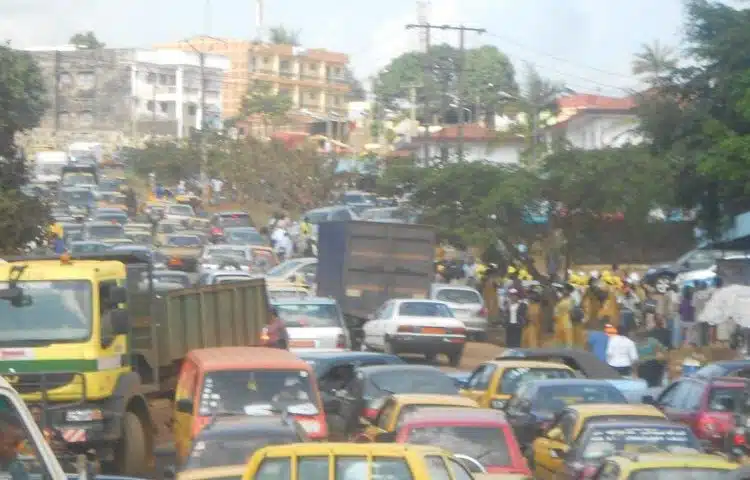
\includegraphics[width=0.5\linewidth]{Images/Embouteillage.png}
    \caption{Embouteillages - Yaoundé}
    \label{fig:embouteillage}
    \cite{camerounCirculation}
\end{figure}

Or une plate-forme permettant au conducteurs de s'orienter dans les directions optimales pour équilibrer le flux de circulation et par ce fait leur temps de trajet, ferait bien l'affaire de ces étudiants et des citoyens de Yaoundé en général, voir des grandes villes du monde.

Analysons maintenant les corrélations d'une telle solution avec les acteurs déjà présents dans le société.


\section{Environnement technique techniques}

\paragraph{\textbf{Les infrastructures}}\\
\begin{itemize}
    \item Cloud computing pour la scalabilité et la flexibilité.
    \item Big data pour l'analyse des données de trafic et de mobilité.
    \item Intelligence artificielle pour l'optimisation des itinéraires et la prédiction du trafic.
    \item Blockchain pour la sécurisation des transactions et la lutte contre la fraude.
\end{itemize}
\paragraph{\textbf{Plateformes}}\\
\begin{itemize}
    \item Plateformes ouvertes et interopérables pour faciliter l'intégration avec les systèmes existants.
    \item API pour permettre aux développeurs de créer des applications et des services innovants.
\end{itemize}
\paragraph{\textbf{Outils}}
\begin{itemize}
    \item Outils de développement open source pour réduire les coûts et favoriser l'innovation.
    \item Outils de sécurité pour protéger les données des utilisateurs.
\end{itemize}
\paragraph{\textbf{Compétences}}
\begin{itemize}
    \item Développeurs logiciels expérimentés dans les technologies cloud, big data et IA.
    \item Data scientists pour l'analyse des données de trafic et de mobilité.
    \item Experts en sécurité pour protéger les données des utilisateurs.
\end{itemize}

La mise en place d'un environnement technique adéquat est essentielle pour le 
développement et la croissance du sous-secteur de la gestion d'itinéraires. Cet environnement doit être basé sur des technologies ouvertes, interopérables et sécurisées, et doit être accessible aux développeurs et aux entrepreneurs.



\section{impulsion du sous secteur}


Pour stimuler le sous-secteur de la gestion des itineraires et du transport au
 Cameroun, plusieurs mesures peuventˆ etre prises pour favoriser son développement
 et son adoption :

 \subsection{L'IA}

\begin{itemize}
    \item \textbf{Prédiction de la demande :} En analysant les données historiques de déplacement et les tendances de comportement des utilisateurs, l'IA peut prédire avec précision les périodes de pointe et les zones à forte demande, permettant ainsi une meilleure planification des services de transport et une allocation optimale des ressources.
    
    \item \textbf{Personnalisation des recommandations :} En utilisant des techniques d'apprentissage automatique, l'IA peut analyser les préférences individuelles des utilisateurs et leur comportement de déplacement pour fournir des recommandations personnalisées, telles que des itinéraires alternatifs, des modes de transport préférés et des offres spéciales.
\end{itemize}
\subsection{Big Data}

\begin{itemize}
    \item \textbf{Analyse des tendances de mobilité :} En recueillant et en analysant de grandes quantités de données sur les déplacements des utilisateurs, le Big Data peut nous aider à comprendre les tendances de mobilité dans la ville, y compris les zones à forte densité de trafic, les horaires de pointe et les schémas de déplacement.
    
    \item \textbf{Prédiction de la demande :} En utilisant des techniques avancées d'analyse prédictive, le Big Data peut nous aider à prévoir la demande future de services de transport, en tenant compte des facteurs tels que les événements spéciaux, les tendances saisonnières et les variations de comportement des utilisateurs.
\end{itemize}

\subsection{Partenariats avec les autorités locales}
L'établissement  des partenariats avec les autorités locales, telles que les municipalités et les gouvernements régionaux, pour partager des données sur les infrastructures de transport, les plans d'urbanisme et les politiques de mobilité. Ces partenariats peuvent nous aider à mieux comprendre les besoins et les défis locaux en matière de transport, ainsi qu'à obtenir un soutien politique et financier pour notre projet.

\subsection{Collaboration avec les entreprises privées}
La collaboration  avec des entreprises privées, telles que les opérateurs de transport, les sociétés de technologie et les fournisseurs de services de mobilité, pour partager des ressources et des expertises. Par exemple, nous pourrions travailler avec des entreprises de technologie pour développer des solutions logicielles avancées, ou avec des opérateurs de transport pour intégrer notre application dans leurs services existants.



\section{impulsion du sous secteur}


Pour stimuler le sous-secteur de la gestion des itineraires et du transport au
 Cameroun, plusieurs mesures peuventˆ etre prises pour favoriser son développement
 et son adoption :

 \subsection{L'IA}

\begin{itemize}
    \item \textbf{Prédiction de la demande :} En analysant les données historiques de déplacement et les tendances de comportement des utilisateurs, l'IA peut prédire avec précision les périodes de pointe et les zones à forte demande, permettant ainsi une meilleure planification des services de transport et une allocation optimale des ressources.
    
    \item \textbf{Personnalisation des recommandations :} En utilisant des techniques d'apprentissage automatique, l'IA peut analyser les préférences individuelles des utilisateurs et leur comportement de déplacement pour fournir des recommandations personnalisées, telles que des itinéraires alternatifs, des modes de transport préférés et des offres spéciales.
\end{itemize}
\subsection{Big Data}

\begin{itemize}
    \item \textbf{Analyse des tendances de mobilité :} En recueillant et en analysant de grandes quantités de données sur les déplacements des utilisateurs, le Big Data peut nous aider à comprendre les tendances de mobilité dans la ville, y compris les zones à forte densité de trafic, les horaires de pointe et les schémas de déplacement.
    
    \item \textbf{Prédiction de la demande :} En utilisant des techniques avancées d'analyse prédictive, le Big Data peut nous aider à prévoir la demande future de services de transport, en tenant compte des facteurs tels que les événements spéciaux, les tendances saisonnières et les variations de comportement des utilisateurs.
\end{itemize}

\subsection{Partenariats avec les autorités locales}
L'établissement  des partenariats avec les autorités locales, telles que les municipalités et les gouvernements régionaux, pour partager des données sur les infrastructures de transport, les plans d'urbanisme et les politiques de mobilité. Ces partenariats peuvent nous aider à mieux comprendre les besoins et les défis locaux en matière de transport, ainsi qu'à obtenir un soutien politique et financier pour notre projet.

\subsection{Collaboration avec les entreprises privées}
La collaboration  avec des entreprises privées, telles que les opérateurs de transport, les sociétés de technologie et les fournisseurs de services de mobilité, pour partager des ressources et des expertises. Par exemple, nous pourrions travailler avec des entreprises de technologie pour développer des solutions logicielles avancées, ou avec des opérateurs de transport pour intégrer notre application dans leurs services existants.

\section{Ressources et contraintes}

\subsection{Ressources}

\subsubsection*{Ressources humaines}
L'application aura besoin d'une équipe dédiée, comprenant des développeurs logiciels, des data scientists, des experts en sécurité, des ingénieurs réseau, et des chefs de projet.

\subsubsection*{Ressources financières}
Différentes sources de financement seront nécessaires, notamment des financements publics et privés, le crowdfunding et des subventions. Des ressources financières supplémentaires peuvent être allouées spécifiquement pour l'hébergement de l'application.

\subsubsection*{Ressources techniques}
L'infrastructure cloud, les plateformes open source et les outils de développement seront essentiels pour le développement et le déploiement de l'application.

\subsubsection*{Données}
L'application aura besoin d'accéder à diverses données, y compris des données de trafic, des données de mobilité et des données cartographiques pour fournir des fonctionnalités précises de gestion et de parcours d'itinéraires.

\subsection{Contraintes}

\subsubsection*{Contraintes fonctionnelles}
\begin{itemize}
    \item \textbf{Interopérabilité :} La solution doit être interopérable avec les systèmes existants.
    \item \textbf{Scalabilité :} La solution doit pouvoir être scalable pour répondre à la croissance du nombre d'utilisateurs.
    \item \textbf{Sécurité :} La solution doit être sécurisée pour protéger les données des utilisateurs.
    \item \textbf{Accessibilité :} La solution doit être accessible à tous les citoyens, y compris les personnes handicapées.
\end{itemize}

\subsubsection*{Contraintes non fonctionnelles}
\begin{itemize}
    \item \textbf{Performance :} La solution doit être performante et offrir un temps de réponse acceptable.
    \item \textbf{Fiabilité :} La solution doit être fiable et disponible 24h/24 et 7j/7.
    \item \textbf{Maintenabilité :} La solution doit être facile à maintenir et à mettre à jour.
    \item \textbf{Évolutivité :} La solution doit être évolutive pour pouvoir s'adapter aux nouveaux besoins et aux nouvelles technologies.
\end{itemize}

 \section{Aspects de régulation, Contraintes opérationnelles \& Pistes de solution digitale}

La mise sur pied d'une telle plate-forme de gestion des itinéraires et plus généralement de gestion du trafic routier dans la ville de Yaoundé, devra se conformer à certains aspects de régulation et à des contraintes opérationnelles.

\subsection{Aspects de régulation}

La solution envisagée durant toute l'analyse qui précède, devra se conformer aux régulations fixées par le gouvernement camerounais, lesquelles régulations sont présentées ci-dessous.

\subsubsection*{Loi sur les communications électroniques}

\begin{itemize}
  \item \textbf{Sécurité des réseaux} : Assurer la protection des infrastructures critiques contre les cyberattaques.
  \item \textbf{Confidentialité des communications} : Garantir la confidentialité des échanges et des données transitant par les réseaux.
  \item \textbf{Accès équitable} : Fournir un accès non discriminatoire aux services de télécommunication.
\end{itemize}

\subsubsection*{Loi sur la protection des données personnelles}
\begin{itemize}
  \item \textbf{Consentement} : Recueillir le consentement explicite des utilisateurs pour la collecte et le traitement de leurs données.
  \item \textbf{Droit à l'oubli} : Permettre aux utilisateurs de supprimer leurs données personnelles sur demande.
  \item \textbf{Transparence} : Informer clairement les utilisateurs sur l'utilisation de leurs données.
\end{itemize}

\subsubsection*{Réglementations relatives aux transports}
\begin{itemize}
  \item \textbf{Licences d'exploitation} : Obtenir les autorisations nécessaires pour opérer des services de transport public.
  \item \textbf{Normes de sécurité} : Respecter les normes de sécurité pour la protection des passagers.
  \item \textbf{Intégration des services} : Assurer l'intégration avec les systèmes de transport public existants.
\end{itemize}

\subsubsection*{}
Ces réglementations sont tirées des lois suivantes:

\begin{itemize}
  \item \textbf{LOI N°2010/013 DU 21 DÉCEMBRE 2010} régissant les communications électroniques au Cameroun, qui établit le cadre pour l'exploitation des réseaux de communications électroniques et la fourniture de services.\cite{Loi2010013}
  \item \textbf{LOI N°2015/006 DU 20 AVRIL 2015} modifiant certaines dispositions de la loi précédente, notamment en ce qui concerne les définitions et les domaines de concession.\cite{cameroon_law_2015}
  \item Et de la réglementation du transport routier au Cameroun.\cite{securoute2024}
\end{itemize}

\subsection{Contraintes Opérationnelles}

En plus des régulations présentées plus haut, cette innovation devra faire face à certaines contraintes du terrain entre autres:

\subsubsection*{Gestion des Crises}
La gestion des crises nécessite une approche pro-active et réactive pour assurer la continuité des services de l'application en cas d'événements imprévus.

\begin{itemize}
    \item Pro-activité: Prévoir des scénarios de crise et élaborer des plans d'intervention.
    \item Réactivité: Mettre en place des systèmes d'alerte rapide et des procédures d'urgence.
\end{itemize}

\subsubsection*{Concurrence}
La concurrence sur le marché peut influencer la stratégie et les fonctionnalités de l'application.
\begin{itemize}
    \item Analyse du marché: Évaluer les offres concurrentes pour identifier les avantages compétitifs.
    \item Innovation: Proposer des fonctionnalités uniques et améliorer l'expérience utilisateur.
\end{itemize}

\subsubsection*{Gestion des Routes}
L'application doit pouvoir s'adapter aux changements dynamiques des conditions routières.
\begin{itemize}
    \item Flexibilité: Intégrer des données en temps réel pour la mise à jour des itinéraires.
    \item Collaboration: Travailler avec les autorités locales pour obtenir des informations précises.
\end{itemize}

\subsubsection*{Coût de l'infrastructure}
Le déploiement de l'application implique des investissements non négligeables en termes d'infrastructure, à l'égard d'un serveur de donnée et des modèles de Big Data pour l'analyse des données.
\begin{itemize}
    \item Budget: Planifier un budget détaillé pour les dépenses en infrastructure.
    \item Financement: Rechercher des sources de financement, telles que des partenariats ou du crowdfunding.
\end{itemize}

\subsection*{Compétences Requises}
Le développement et la gestion de l'application exigent des compétences techniques pointues et une expertise en gestion de projet.
\begin{itemize}
    \item Développement logiciel: Maîtrise des langages de programmation tels que Java, Python, et des frameworks de développement mobile.
    \item Analyse de données: Compétences en traitement et analyse de données massives (Big Data), utilisation d'outils comme Hadoop ou Spark.
    \item \textbf{Gestion de projet}: Expérience en méthodologies agiles et outils de gestion de projet comme JIRA.
    \item \textbf{Cybersécurité}: Connaissance approfondie des protocoles de sécurité et des meilleures pratiques pour protéger les données des utilisateurs.
\end{itemize}

\subsubsection*{Résistance au Changement}
Les utilisateurs peuvent hésiter à adopter une nouvelle technologie.
\begin{itemize}
    \item Sensibilisation: Mener des campagnes pour éduquer les utilisateurs sur les avantages de l'application.
    \item Support: Offrir un support technique et une assistance utilisateur pour faciliter la transition.
\end{itemize}

\subsection{Solutions Digitales pour la Gestion des Réglementations et Contraintes Opérationnelles}

\subsubsection*{Plate-forme de Gestion Intégrée}
Une plate-forme en ligne centralisée utilisant des API pour intégrer différentes données de transport, réglementations et contraintes opérationnelles.

\subsubsection*{Utilisation de la Blockchain}
Application de la technologie blockchain pour assurer la transparence et la traçabilité des transactions et des opérations liées au transport.

\subsubsection*{Big Data et Analytique Avancée}
Utilisation de Big Data pour analyser les tendances de mobilité et optimiser les itinéraires en temps réel, tout en respectant les réglementations en vigueur.

\subsubsection*{Systèmes de Sécurité et de Conformité}
Développement de systèmes automatisés pour surveiller et garantir le respect des normes de sécurité et des lois fiscales applicables.
\\
Étant d'ores et déjà au parfum des contraintes et réglementations auxquelles cette solution devra se conformer, plus rien ne nous empêche d'aller vers la modélisation mathématique de ladite solution.


\section{Modélisation mathématique du problème}
Notre modelisation mathematique commence par le choix des outils mathematiques utilises ( \textbf{les graphes} ),
passe par le formalisme et les analogies et se terminent par le choix des algorithmes permettant de resourdre le probleme.\\

Cependant,justifons d'abord le choix de la \textbf{theorie des graphes}
\begin{enumerate}
    \item Tout d'abord,nous devons souligner que la theorie des graphes est un outil simple,facile a comprendre et qui illustre mieux comment representer une carte,des routes et autres.
    \item De plus,le probleme que nous devons resourdre s'assimile directemnet aux poblemes de parcours en  theorie des graphes
    \item par ailleurs,La théorie des graphes offre des outils puissants pour modéliser les connexions entre les différents points du réseau routier et les déplacements des véhicules d'un point à un autre.
\end{enumerate}




% ------------------------------------------------------
\subsection{Un peu de théorie des graphes}
A fin de faciliter la comprehension de notre modele,nous allons bievrement definir expliquer les concepts de base de la theorie des graphes utiles pour notre modelisation. 

\begin{figure}[h]
    \centering
    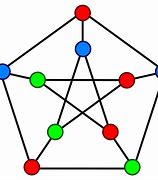
\includegraphics[width=0.5\linewidth]{Images/Theory.jpeg}
    \caption{La theorie des graphes}
    \label{fig:un peu de theorie des graphes}
    \cite{graph_image}
\end{figure}


\subsubsection{Qu'est ce que de théorie des graphes ?}

La théorie des graphes est une branche des mathématiques qui étudie les relations entre les objets. Les objets sont représentés par des points, appelés sommets, et les relations entre eux sont représentées par des lignes, appelées arêtes. Voici quelques concepts de base :

\subsubsection{Terminologie}

\begin{itemize}
    \item \textbf{Graphe :} Ensemble de sommets et d'arêtes.
    \item \textbf{Sommets (ou nœuds) :} Les points d'un graphe.
    \item \textbf{Arêtes :} Les lignes reliant les sommets.
    \item \textbf{Graphe orienté :} Un graphe dans lequel les arêtes ont une direction.
    \item \textbf{Graphe non orienté :} Un graphe dans lequel les arêtes n'ont pas de direction.
    \item \textbf{Graphe mixte :} Un graphe dans lequel certaines arêtes peuvent être orientées et d'autres non, et où les sommets peuvent être attribués à différents types ou classes.
    \item \textbf{Graphe pondéré :} Un graphe dans lequel chaque arête est associée à un poids ou une valeur. Ces poids peuvent représenter des distances, des coûts, des temps, etc., et sont utilisés pour optimiser les algorithmes de recherche de chemins tels que Dijkstra et A* qui seront presentes ci bas.
\end{itemize}


\begin{figure}[h]
    \centering
    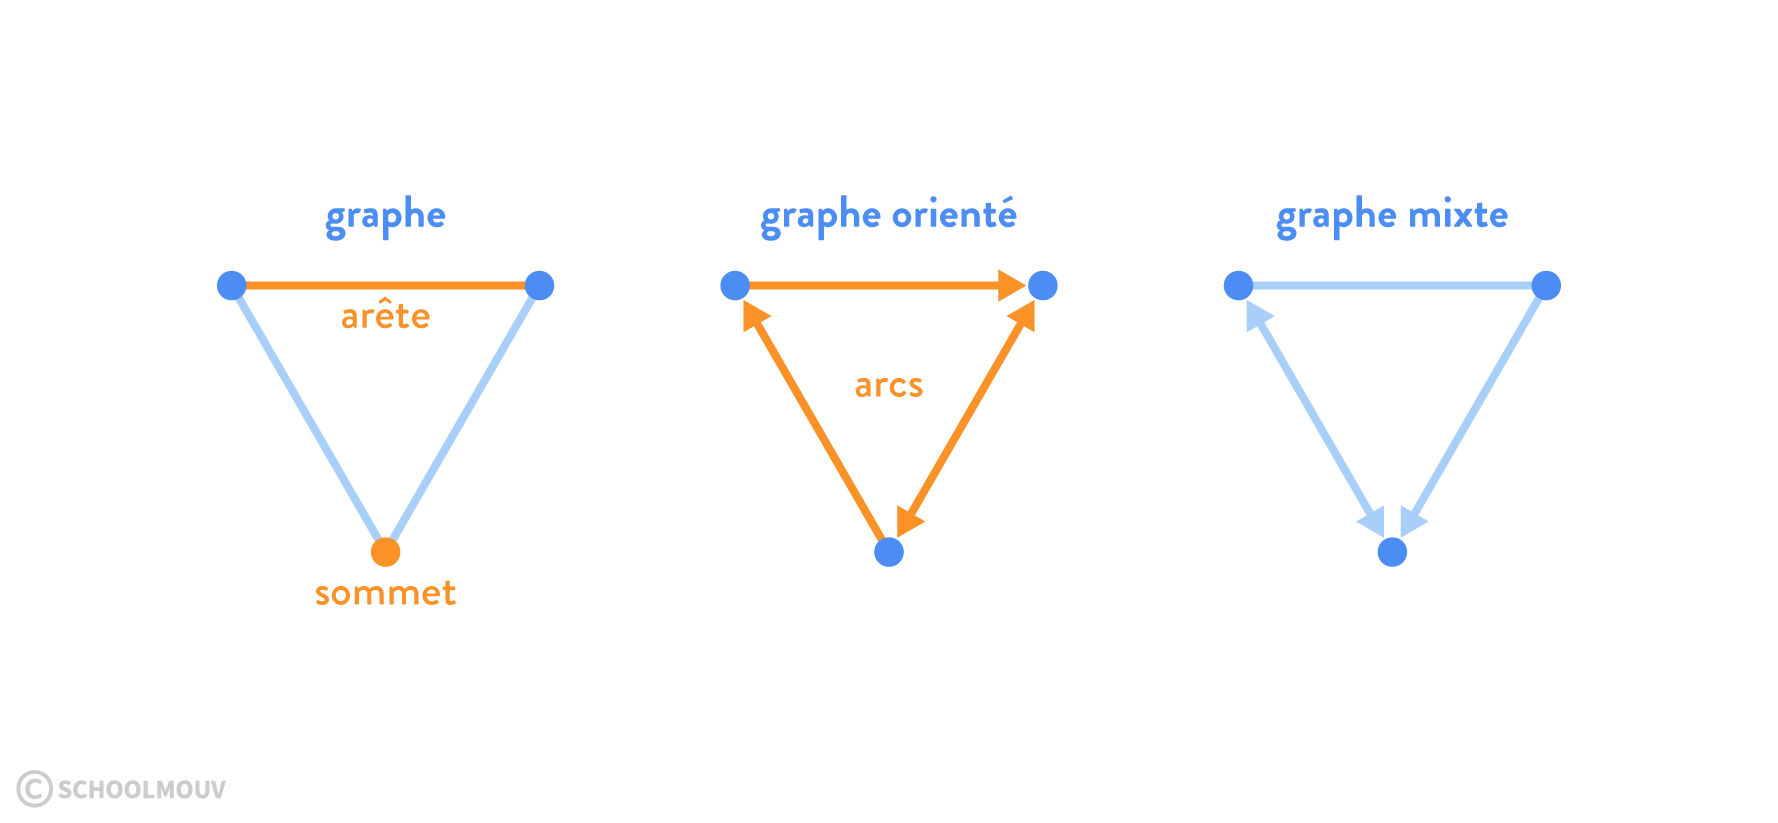
\includegraphics[width=0.9\linewidth]{Images/sommets.png}
    \caption{Terminologie theorie des graphes}
    \cite{graph_image2}
\end{figure}

\newpage
\subsubsection{Types de graphes}

Il existe plusieurs types de graphes, dont les plus courants sont :

\\
     \textbf{Graphe simple :} Un graphe sans boucles ni arêtes multiples entre les mêmes sommets.
\begin{figure}[h]
    \centering
    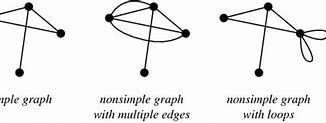
\includegraphics[width=0.4\linewidth]{Images/simple_graph.jpeg}
    \caption{graphe simple}
    \cite{graph_image3}
    \end{figure}
     
  \\   \textbf{Graphe complet :} Un graphe dans lequel chaque paire de sommets est reliée par une arête.

    \begin{figure}[h]
    \centering
    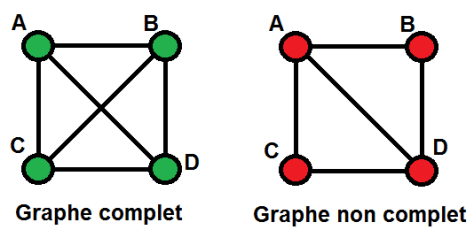
\includegraphics[width=0.4\linewidth]{Images/graph_simple_complet.png}
    \caption{graphe complet}
    
    \cite{graph_image4}
\end{figure}
    
  \\  \textbf{Graphe biparti :} Un graphe dont les sommets peuvent être divisés en deux ensembles disjoints, et où chaque arête relie un sommet d'un ensemble à un sommet de l'autre ensemble.

\begin{figure}[h]
    \centering
    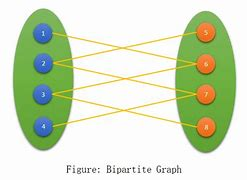
\includegraphics[width=0.4\linewidth]{Images/bipartite_graph.jpeg}
    \caption{graphe bipartite}
    % \cite{graph_image5}
\end{figure}





La théorie des graphes offre de nombreux outils et concepts pour modéliser et résoudre une variété de problèmes dans divers domaines, tels que les réseaux sociaux, les réseaux informatiques, les itinéraires de transport, etc.




\newpage
% ------------------------------------------------------
\subsection{Formalisme et modelisation de l'environnement}
A fin de mieux modeliser notre probleme,nous allons faire une analogie avec \textbf{la theorie des graphes}.Ainsi,les entites principales de notre carte sont:

\begin{itemize}
    \item \textbf{Les points d'arret:} qui representent simplement les differents points d'arret d'un vehicules/clients sur une carte.Il
    s'agit des carrefours,stations services,pharmacies,restaurants,bars qui pourraient servir de destination dans une ville donnee.
      \item \textbf{Les routes} qui representent simplent les liens entre ces points,une route peut etre vue comme un support permettent de se deplacer d'un point a un autre
    \item \textbf{les itineraires} qui representent simplement des  sucsessions ordonnes  de routes peremttant d'aller d'un poin a un autre.
    \textbf{les contraintes} comme \textbf{le distance,le temps,la rigueur d'une route,l'encombrement,....}
      
\end{itemize}

Maintenant ,voici notre facon de modeliser ces entites:
\begin{itemize}
      \item \textbf{Notre carte} sera assimillee a \textbf{ un graphe} mathematique.
        \item \textbf{Les points d'arret} seront assimiles aux\textbf{ sommets} du graphe.
          \item \textbf{Les routes} seront vues ici de facon basique comme des \textbf{arretes} et des \textbf{chemins sur le graphe}.\textbf{le deplacment sur une route est vu comme une relation entre 2 sommets}
            \item \textbf{les itineraires} seront simplement vus comme une succession de points lies.IL s'agira simplement d'une notion assimilable a une route mais un peu plus large.
              \item \textbf{les contaraintes sur une route} serviront ici a construire \textbf{le poids du chemin correspondant}.A chaque fois, en fonction des contraintes utilisees pour un filtre de recherche,nous construirons une metrique composite des contraintes associees qui permettra de definir le poids du chemin. 
\end{itemize}
Dans cette lancee,notre probleme de gestion et de parcours d'itineraire se ramene simplement au probleme de \textbf{gestion et parcours d'un graphe en mathematique.}

\newpage
% ------------------------------------------------------

\subsection{Algorithmes de Parcours d'un Graphe}

les differents facteurs nous permettant de choisir les algorithmes de parcours de notre graphe sont:
\begin{itemize}
    \item \textbf{l'architechture reseau de la ville de yaounde:} en effet la ville de yaounde a une architechture reseau en etoile centree.
    \item \textbf{les besoins de parcours lies aux filtres de recherches} tel que la distance,l'optimalite,l'encombrement.
    \item \textbf{les contraintes d'equite:} pour eviter que les clients se dirigent tous vers le meme lieu au meme moment. 
\end{itemize}

\begin{figure}[h]
    \centering
    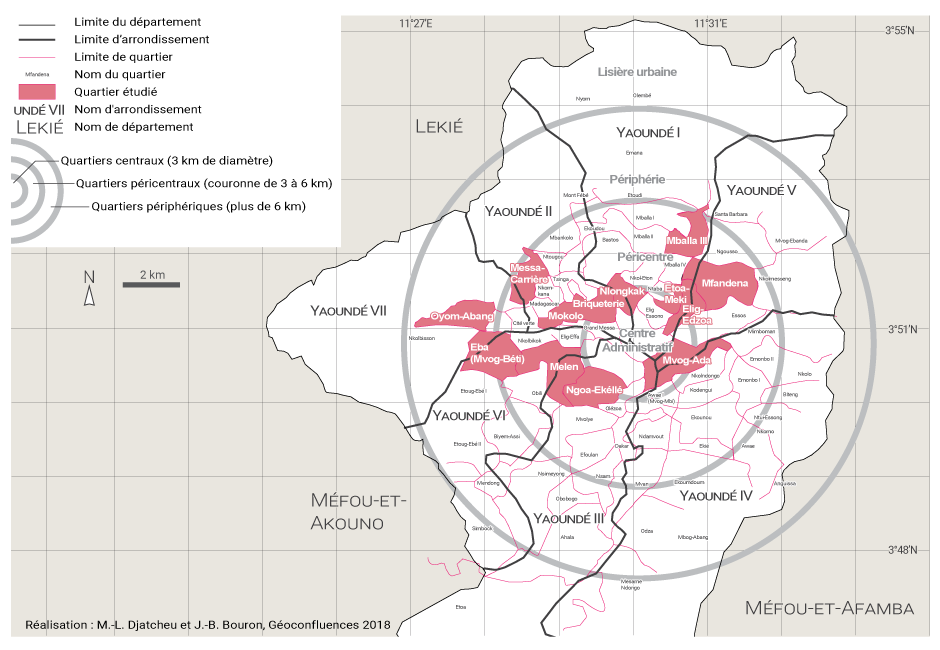
\includegraphics[width=0.8\linewidth]{Images/localisation-yaounde.png}
    \caption{architechture reseau ville de yaounde}
\end{figure}

\newpage
-Parlons maintenant des differents algorithmes de parcours qui nous interessent:
\subsubsection*{Parcours en Largeur (BFS - Breadth First Search)}
\begin{itemize}
    \item \textbf{Principe} : Le BFS explore les nœuds du graphe en utilisant un ordre de visite en largeur. Il commence par le nœud de départ, puis visite tous ses voisins avant de passer aux voisins de ces voisins, et ainsi de suite.
    \item \textbf{Spécificités} :
        \begin{itemize}
            \item Utilise une file (FIFO) pour gérer l'ordre de visite des nœuds.
            \item Trouve le plus court chemin entre deux nœuds non pondérés.
            \item Convient pour la recherche de la solution la plus rapide.
        \end{itemize}
\end{itemize}

\begin{figure}[h]
    \centering
    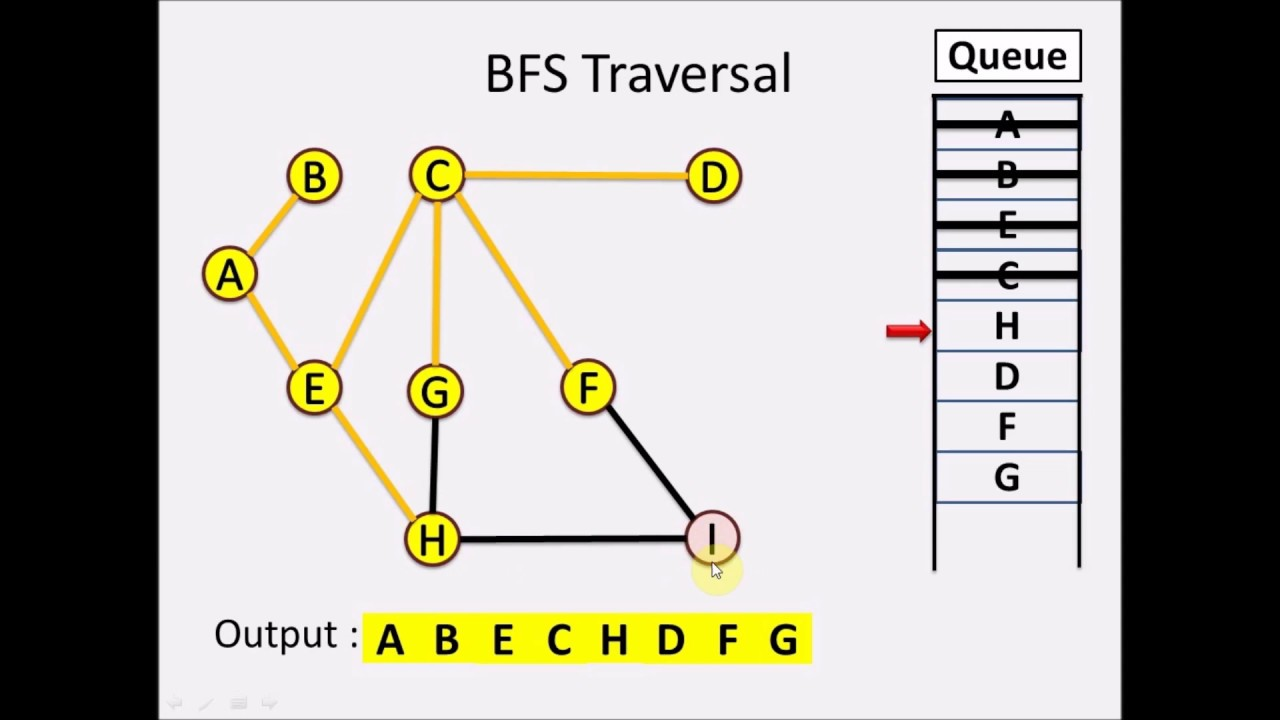
\includegraphics[width=0.5\linewidth]{Images/BFS.jpeg}
    \caption{algorithme BFS}
\end{figure}


\subsubsection*{Parcours en Profondeur (DFS - Depth First Search)}
\begin{itemize}
    \item \textbf{Principe} : Le DFS explore les nœuds du graphe en utilisant la récursivité. Il visite les nœuds les plus "profonds" en premier, puis remonte progressivement dans le graphe.
    \item \textbf{Spécificités} :
        \begin{itemize}
            \item Utilise la pile (LIFO) pour gérer l'ordre de visite des nœuds.
            \item Peut être utilisé pour détecter des cycles dans un graphe.
            \item Ne garantit pas le plus court chemin.
        \end{itemize}
\end{itemize}

\begin{figure}[h]
    \centering
    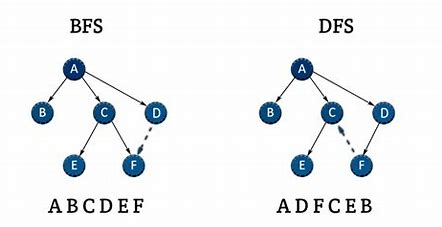
\includegraphics[width=0.5\linewidth]{Images/DFS.jpeg}
    \caption{algorithme DFS}
\end{figure}

\subsubsection*{Algorithme de Dijkstra}
\begin{itemize}
    \item \textbf{Principe} : L'algorithme de Dijkstra permet de trouver le plus court chemin entre deux sommets d'un graphe (orienté ou non orienté). Il choisit le sommet non visité avec la distance la plus faible, calcule la distance à travers lui pour chaque voisin non visité, et met à jour la distance du voisin si elle est plus petite.
    \item \textbf{Spécificités} :
        \begin{itemize}
            \item Utilise un tableau de mémoire pour garder en mémoire les distances minimisées.
            \item Convient pour les graphes orientés pondérés par des réels positifs.
            \item Peut également calculer un plus court chemin entre un sommet de départ et un sommet d'arrivée.
        \end{itemize}
\end{itemize}

\begin{figure}[h]
    \centering
    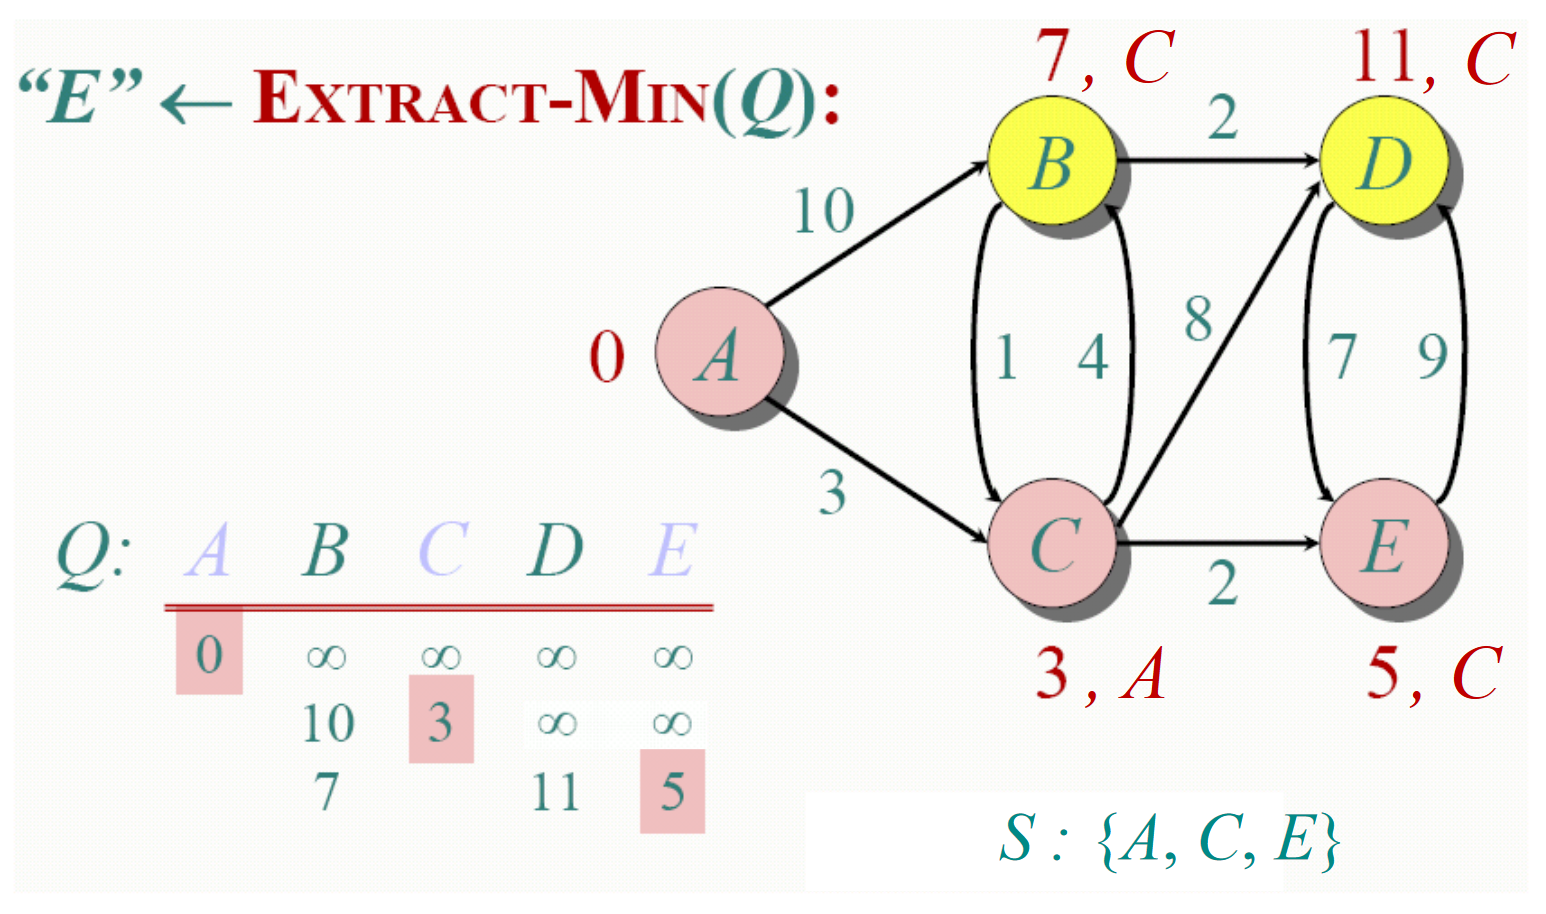
\includegraphics[width=0.5\linewidth]{Images/djiskra.png}
    \caption{Algorithme de Dijkstra}
\end{figure}

\subsubsection*{Algorithme A*}

\begin{figure}[h]
    \centering
    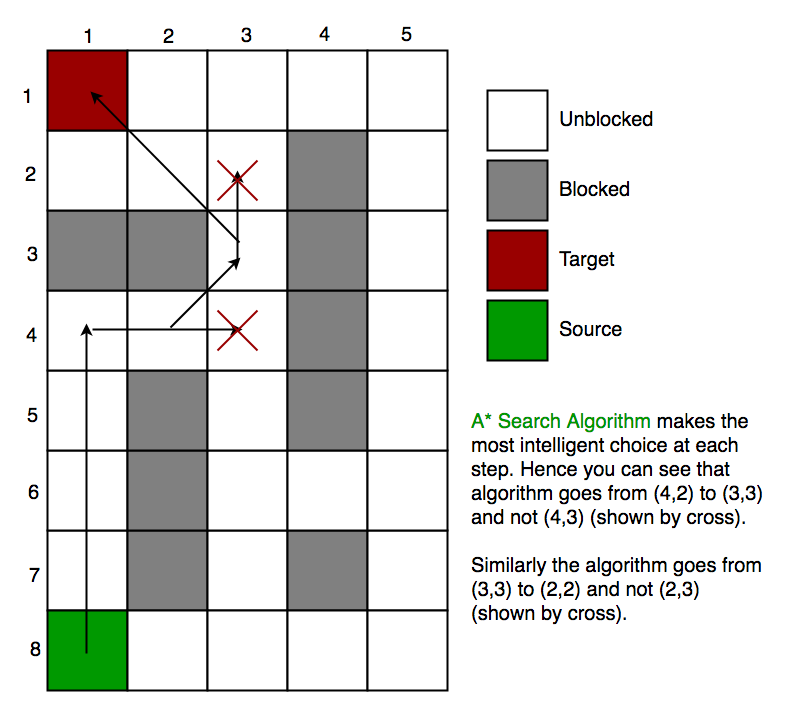
\includegraphics[width=0.5\linewidth]{Images/a_-search-algorithm-2.png}
    \caption{Algorithme A*}
\end{figure}

\begin{itemize}
    \item \textbf{Principe} : L'algorithme A* utilise une fonction heuristique pour estimer le coût restant à parcourir pour atteindre le sommet cible à partir du sommet actuel. Il combine cette estimation avec le coût réel parcouru jusqu'à présent pour évaluer les sommets à explorer en priorité. A* explore les sommets avec le coût total le plus faible en priorité.
    \item \textbf{Spécificités} :
        \begin{itemize}
            \item Utilisation d'une fonction heuristique : L'algorithme A* utilise une fonction heuristique qui fournit une estimation du coût restant pour atteindre le sommet cible. Cette fonction doit être admissible (ne jamais surestimer le coût restant) pour garantir l'optimalité de l'algorithme.
            \item Efficace pour la recherche de chemins dans les graphes avec des coûts non uniformes : L'algorithme A* peut être plus efficace que Dijkstra dans les graphes où les coûts des arêtes varient et nécessitent une exploration plus intelligente.
        \end{itemize}
\end{itemize}


En résumé, le choix de l'algorithme dépend du problème spécifique que vous essayez de résoudre. Le BFS est idéal pour les chemins les plus courts, tandis que le DFS est plus souple pour explorer toutes les possibilités. L'algorithme de Dijkstra est puissant et polyvalent pour résoudre les problèmes de plus court chemin. L'algorithme A*, quant à lui, offre une approche efficace pour trouver des chemins dans les graphes avec des coûts non uniformes, en utilisant une fonction heuristique pour guider la recherche. Celui que nous allons souvent utiliser dépendra à chaque fois de la tâche que nous voudrons accomplir lors de la gestion des sommets sur notre graphe.










\section{Résultats}
% Présentation des résultats obtenus dans le cadre du projet
Les résultats de ce projet sont les suivants :
\begin{itemize}
    \item Résultat 1 : [Description du résultat 1]
    \item Résultat 2 : [Description du résultat 2]
    \item ...
\end{itemize}
I'm
\section{Discussion}
% Discussion des résultats et de leur importance
Les résultats obtenus ont permis de conclure que [résumé des conclusions]. Ces résultats sont importants car ils [raison de l'importance des résultats].

\section{Difficultés rencontrées}

Nous avons rencontré plusieurs défis tout au long de cette étude. Parmi les principales difficultés, nous pouvons citer :

\begin{enumerate}
    \item \textbf{Accès aux données :} Obtenir des données précises et complètes sur la mobilité urbaine et les statistiques de transport dans la ville de Yaoundé s'est avéré être un défi majeur. issue du fait qu'il y es pas assez d'tude sur le sujet
    
    \item \textbf{Analyse de la complexité du système :} La mobilité urbaine est un domaine complexe, impliquant de nombreux acteurs et facteurs interdépendants. Comprendre et modéliser cette complexité pour proposer des solutions efficaces nécessitait une analyse approfondie et une expertise multidisciplinaire.
    
    \item \textbf{Contraintes de temps :} Le temps limité pour mener à bien cette étude a constitué un autre défi. Nous avons dû concilier les exigences du projet avec d'autres obligations académiques et professionnelles, ce qui a parfois entravé notre progression et notre capacité à approfondir certaines questions.
    
    \item \textbf{Disponibilité des ressources :} Les ressources techniques et financières limitées ont également été un obstacle. Pour mettre en œuvre certaines solutions proposées, nous aurions eu besoin de ressources supplémentaires, telles que des logiciels spécialisés, du matériel informatique ou un financement pour la collecte de données sur le terrain.
    
    \item \textbf{Appréhension des outils :} La prise en main et la maîtrise des outils tels que OpenStreetMap se sont avérées être des défis supplémentaires. La complexité de ces plateformes et la nécessité de comprendre en profondeur leurs fonctionnalités pour l'analyse des données cartographiques ont demandé du temps et des efforts supplémentaires.
\end{enumerate}


\newpage

\section*{Conclusion}
\addcontentsline{toc}{section}{conclusion}
% Conclusion générale du rapport de projet

Le projet "My Way" s'inscrit dans une démarche visant à répondre efficacement aux défis de la mobilité urbaine à Yaoundé, capitale dynamique du Cameroun. À travers une analyse approfondie de la situation actuelle de la ville, nous avons identifié les principaux obstacles qui entravent la fluidité des déplacements quotidiens de ses habitants. Face à ces défis, la digitalisation du secteur des transports émerge comme une solution prometteuse pour améliorer la qualité de vie des citoyens, optimiser l'efficacité des déplacements et contribuer au développement économique de la région.

La transition vers une approche numérique du transport présente de multiples avantages, tant sur le plan économique que social et environnemental. En exploitant les possibilités offertes par les technologies numériques, telles que les applications mobiles et les systèmes de suivi en temps réel, nous pouvons améliorer la gestion du trafic, réduire les temps de déplacement et minimiser l'impact environnemental des transports. De plus, une plate-forme numérique robuste peut favoriser l'émergence de nouveaux services, tels que le covoiturage et la livraison de colis, répondant ainsi aux besoins diversifiés des utilisateurs.

La transformation digitale du secteur des transports représente également une opportunité pour le Cameroun de renforcer sa compétitivité sur la scène internationale. En investissant dans des infrastructures numériques innovantes, le pays peut positionner Yaoundé comme une ville intelligente et dynamique, capable de répondre aux exigences croissantes de ses habitants et des visiteurs.

En sommes, le projet "My Way" incarne une vision ambitieuse de l'avenir de la mobilité urbaine à Yaoundé. En adoptant une approche holistique et intégrée, nous pouvons transformer les défis actuels en opportunités de développement durable et d'amélioration de la qualité de vie pour tous les citoyens. Avec un engagement continu envers l'innovation et la collaboration, nous pouvons façonner un avenir où les déplacements urbains sont fluides, efficaces et respectueux de l'environnement.
\newpage

\section*{Références}
\addcontentsline{toc}{section}{Références}

\begin{enumerate}
    \item 237online. Cameroun– Embouteillages : 794 milliards FCFA `a lever pour la voie de contournement de Yaound´e. 237online.com. Disponible sur : \url{https://237online.com}. 2022.
    \item Actu Cameroun. “Circulation `a Yaound´e : au rythme des embouteillages”. In : Camer.be (sept. 2016). Publi´e le 29 Sep 2016. url : \url{https://www.actucameroun.com/2016/09/29/circulation-a-yaounde-au-rythme-des-embouteillages/}.
    \item Conseil National de la communication. LOI N°2010 013 DU 21 DECEMBRE 2010 REGISSANT LES COMMUNICATIONS ELECTRONIQUES AU CAMEROUN. T´ el´ echarg´ e depuis le site du CNC- NCC. Acc´ed´e le 28/07/2021. D´ ec. 2010. url : \url{https://www.cnc.cm}.
    \item quizizz library. Th´eorie des graphes- Une Introduction Visuelle. url : \url{https://www.bing.com/images/search?view=detailV2&ccid=gwrBHB2W&id=7C4A38AD4426ACF4C34E9AE114E0A1156DA53F24&thid=OIP.gwrBHB2WMUPSiwGPH36n0AHaHG&mediaurl=https%3a%2f%2fquizizz.com%2fmedia%2fresource%2fgs%2fquizizz-media%2fquizzes%2fea93dd07-ba70-4ece-a80a-464393d2f5ba&cdnurl=https%3a%2f%2fth.bing.com%2fth%2fid%2fR.830ac11c1d.}
    \item mathWorld. Th´eorie des graphes- graphes simples. url : \url{https://www.bing.com/images/search?view=detailV2&ccid=jQoW941E&id=75E91A157A1A3D60C32D3C23C8DEDC007290AB44&thid=OIP.jQoW941EEgEv23h_bRGIigHaCn&mediaurl=https%3a%2f%2fmathworld.wolfram.com%2fimages%2feps-gif%2fSimpleGraph_950.gif&cdnurl=https%3a%2f%2fth.bing.com%2fth%2fid%2fR.8d0a16f78d4412012fdb787f6d11888a%3frik%3dRKuQcgDc3sgjPA%26pid%3dImgRaw%26r%3d0&exph=179&expw=507&q=graphe+simple+vs+graph+non+simple&simid=608032159940963323&FORM=IRPRST&ck=76A0AA8744DDCC8DE44A721228C438C5&selectedIndex=0&itb=0&idpp=overlayview&ajaxhist=0&ajaxserp=0.}
    \item JeanPatrick Mfoulou Olugu.Mobilit´e urbaine et politique de transport `a Yaound´ e. Research Report. ffhal-01315178. Universit´e de Yaound´ e II soa FSEG, 2016.
    \item R´ epublique du Cameroun. LOI N°2015/006 DU 20 AVRIL 2015 MODIFIANT ET COMPLETANT CERTAINES DISPOSITIONS DE LA LOI N°2010/013 DU 21 DECEMBRE2010REGISSANTLESCOMMUNICATIONSELECTRONIQUES AU CAMEROUN. Assembl´ee Nationale et Pr´ esident de la R´ epublique. Avr. 2015. url : \url{https://www.art.cm/sites/default/files/documents/LOI%20N%C2%B0 2015%20006%20DU%2020%20AVRIL%202015%20MODIFIANT%20ET%20COMPLETANT%20 CERTAINES%20DISPOSITIONS%20DE%20LA%20LOI%20%20DE%202010%20LCE.pdf}.
    \item Groupe Logistique Conseil et SECUROUTE. Le transport routier au Cameroun : Recueil et textes. Securoute Africa. Disponible sur : \url{https://www.securouteafrica.org}. 2024.
\end{enumerate}


\end{document}



